\langsection[subsection]{Group Riding}{Езда в группе}


\begin{langblock}{0.425}
	\begin{eng}
	
	If you ride with others, do it in a way that promotes safety and doesn't interfere with the flow of traffic.
	\end{eng}
	\begin{rus}
		
		Если вы едите в группе, делайте это так, чтобы это обеспечивало безопасность и не создавало помех для движению остальному транспорту.
\end{rus}
\end{langblock}




\langsection[subsubsection]{Keep the Group Small}{Малыми группами}


\begin{langblock}{0.425}
	\begin{eng}
	
	Small groups make it easier and safer for car drivers who need to get around them. A small number isn't separated as easily by traffic or red lights. Riders won't always be hurrying to catch up. If your group is larger than four or five riders, divide it up into two or more smaller groups.
	\end{eng}
	\begin{rus}
		
		Автомобилям проще и безопасней обогнать малые группы. Автомобиль или красный свет светофора с меньшей вероятностью разорвет малую группу. Отстающим не надо торопиться чтобы не отстать от группы. Если ваша группа состоит из более чем четырех–пяти участников, разделите ее на две или более группы.
\end{rus}
\end{langblock}


\langsection[subsubsection]{Keep the Group Together}{Езжайте кучно}


\begin{langblock}{0.425}
	\begin{eng}
	
	\begin{itemize}[noitemsep]
		\item Plan --- The leader should look ahead for changes and signal early so the word gets back in plenty of time. Start lane changes early to permit everyone to complete the change.
		\item Put Beginners Up Front --- Place inexperienced riders just behind the leader. That way the more experienced riders can watch them from the back.
		\item Follow Those Behind --- Let the tailender set the pace. Use your mirrors to keep an eye on the person behind. If a rider falls behind, everyone should slow down a little to stay with the tailender.
		\item Know the Route --- Make sure everyone knows the route. Then, if someone is separated they won't have to hurry to keep from getting lost or taking a wrong turn. Plan frequent stops on long rides.
	\end{itemize}
	\end{eng}
	\begin{rus}
		
		\begin{itemize}[noitemsep]
			\item Планируйте заранее "--- Лидер должен предвидеть изменения и подавать сигналы заранее, чтобы сообщение «дошло» с достаточным запасом по времени. Начните смену ряда заранее, чтобы всех успели завершить маневр.
			\item Поставьте новичков вперед "--- Неопытных мотоциклистов сразу за лидером. Так более опытные мотоциклисты смогут присматривать за ними сзади.
			\item Следите за теми, кто едет сзади "--- Пусть темп задает замыкающий. Следите за тем, кто сзади. Если кто-то отстает, всем следует снизить скорость, не растягивать строй и ориентироваться на замыкающего.
			\item Знайте маршрут "--- Убедитесь, что все знают маршрут. Тогда, если кто-то отстанет, ему не придется рискованно торопиться, боясь заблудиться или свернуть не туда. Планируйте интервалы с остановками во время длительных поездок.
		\end{itemize}
\end{rus}
\end{langblock}



\langsection[subsubsection]{Keep Your Distance}{Держите дистанцию}


\begin{langblock}{0.425}
	\begin{eng}
	
	
	Maintain close ranks but at the same time keep a safe distance to allow each rider in the group time and space to react to hazards. A close group takes up less space on the highway, is easier to see and is less likely to be separated. However, it must be done properly.
	
	
	\begin{description}
		\item[Don't Pair Up] Never operate directly alongside another rider. There is no place to go if you have to avoid a car or something on the road. To talk, wait until you are both stopped.
		\item[Staggered Formation] This is the best way to keep ranks close yet maintain an adequate space cushion.
		\item[Single-File Formation] It is best to move into a single-file formation when riding curves, turning, entering or leaving a highway.
	\end{description}
	\end{eng}
	\begin{rus}
		
		
		Группа должна ехать компактно, но при этом соблюдать безопасную дистанцию, чтобы у каждого мотоциклиста в группе был запас времени на реакцию. Плотная группа занимает меньше места на дороге, ее легче заметить, и вероятность ее разрыва меньше. Однако все нужно делать по уму.
		
		
		\begin{description}
			\item[Не ездите бок о бок] Никогда не ездите непосредственно рядом с другим мотоциклистом. Если вам понадобится уклоняться от автомобиля или препятствия на дороге, вам некуда будет сместиться. Чтобы поговорить, дождитесь остановки.
			\item[Шахмотный порядок] Это лучший способ держаться плотной группой, сохраняя при этом достаточный запас для маневра.
			\item[Езда гуськом] Лучше всего переходить в колонну по одному при прохождении поворотов, разворотов, въезде на шоссе или съезде с него.
		\end{description}
\end{rus}
\end{langblock}
	
	
\begin{langblock}{0.425}
	\begin{eng}
		
		The leader rides in the left side of the lane, while the second rider stays one second behind in the right side of the lane.
		
		A third rider maintains in the left position, two seconds behind the first rider. The fourth rider would keep a two-second distance behind the second rider. This formation keeps the group close and permits each rider a safe distance from others ahead, behind and to the sides.
		
		\begin{itemize}[noitemsep]
			\item Passing in Formation --- Riders in a staggered formation should pass one at a time.
			\item First, the lead rider should pull out and pass when it is safe. After passing, the leader should return to the left position and continue riding at passing speed to open room for the next rider.
			\item After the first rider passes safely, the second rider should move up to the left position and watch for a safe chance to pass. After passing, this rider should return to the right position and open up room for the next rider.
		\end{itemize}
	\end{eng}
	\begin{rus}
		Лидер едет по левой стороне полосы движения, а второй мотоциклист держится на расстоянии одной секунды сзади по правой стороне полосы.
		
		Третий мотоциклист держится слева, отставая от первого на две секунды. Четвертый мотоциклист должен соблюдать двухсекундное расстояние от второго. Такая формация позволяет группе держаться вместе и обеспечивает каждому мотоциклисту безопасное расстояние до других участников движения спереди, сзади и по бокам.
		
		\begin{itemize}[noitemsep]
			\item Обгон в группе --- Мотоциклисты, едущие в шахматном порядке, должны обгонять по очереди, по одному.
			\item Сначала лидер должен выехать вперед и совершить обгон, когда это безопасно. После обгона лидер должен встать на левую позицию и продолжить езду со скоростью обгона, чтобы освободить место сзади себя для следующего мотоциклиста.
			\item После того как первый мотоциклист безопасно совершит обгон, второй мотоциклист занимает место лидера, переместившись на левую позицию и выждать подходящий момент для обгона. После обгона этот мотоциклист должен встать на правую позицию и освободить место для следующего мотоциклиста позади себя.
		\end{itemize}
\end{rus}
\end{langblock}




\begin{langblock}{0.425}
	\begin{eng}
	
	Some people suggest that the leader should move to the right side after passing a vehicle. This is not a good idea. It encourages the second rider to pass and cut back in before there is a large enough space cushion in front of the passed vehicle. It's simpler and safer to wait until there is enough room ahead of the passed vehicle to allow each rider to move into the same position held before the pass.
	\end{eng}
	\begin{rus}
		
		Некоторые предлагают, чтобы лидер после обгона перемещался в правую сторону. Это так себе идея. Такой подход побуждает второго мотоциклиста совершать обгон и возвращаться в колонну до того, как перед обгоняемым транспортным средством образуется достаточно большой запас пространства. Проще и безопаснее подождать, пока перед обгоняемым транспортным средством не появится достаточно места, чтобы каждый мотоциклист мог вернуться на ту же позицию, которую занимал до обгона.
\end{rus}
\end{langblock}






\begin{figure}[htbp]
	\begin{subfigure}{0.45\textwidth}	
		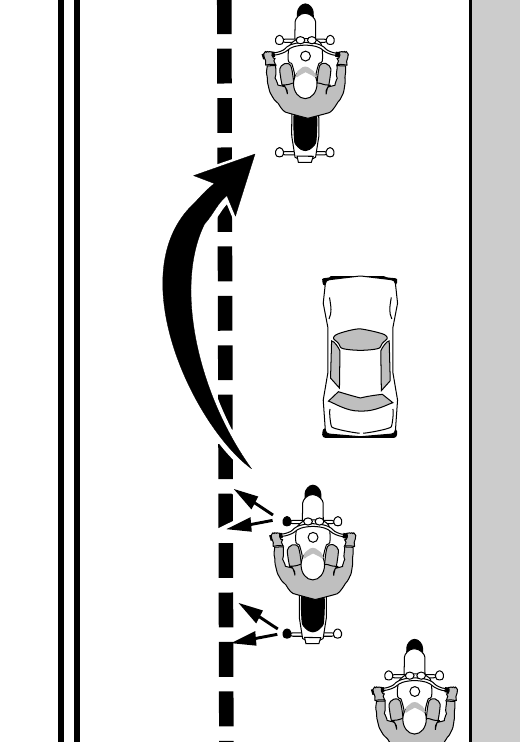
\includegraphics[width=0.95\textwidth, frame]{images/gr_pass_1.png}
		\caption{Stage 1}
		\label{fig:gr_pass_1}
	\end{subfigure}
	\hspace*{\fill}
	\begin{subfigure}{0.42\textwidth}
		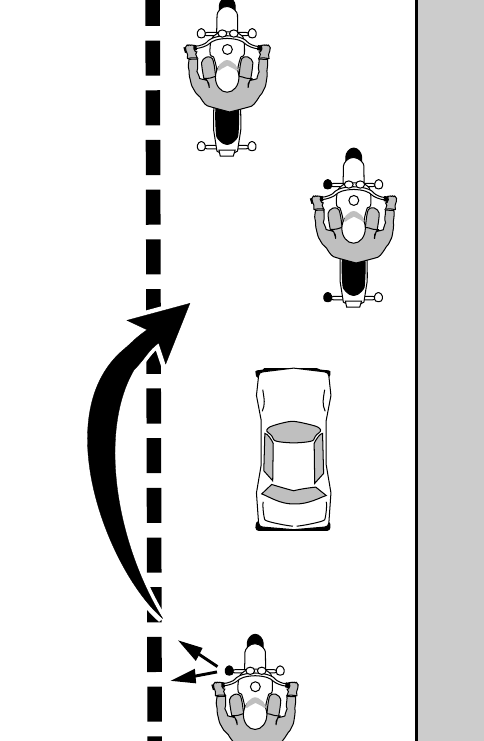
\includegraphics[width=0.95\textwidth, frame]{images/gr_pass_2.png}
		\caption{Stage 2}
		\label{fig:gr_pass_2}
	\end{subfigure}
	
	\caption{Group passing}
\end{figure}











